\documentclass[french]{article}
\usepackage[T1]{fontenc}
\usepackage[utf8]{inputenc}
\usepackage{lmodern}
\usepackage[a4paper]{geometry}
\usepackage{babel}
\usepackage{amsmath}
\usepackage{amsfonts}
\usepackage{tcolorbox}
\usepackage{color}
\usepackage{breqn}

\begin{document}
	\title{DM2}
	\date{Dernière modification \today}
	
	\maketitle
	
	\subsection*{Exercice 1}
	
	\begin{tcolorbox}[colback=red!5!white,colframe=red!75!black]
		Considérons l'équation différentielle $\dot{X} = f(X)$ où $f : \mathbb{R}^N \to \mathbb{R}^N$ est de classe $\mathcal{C}^1$.
		
		Pour tout $Z_0 \in \mathbb{R}^N$, on note $T_{max}(Z_0) > 0$ le temps d'existence maximal de la solution $Z(t)$ de l'équation différentielle $\dot{Z} = f(Z)$ de donnée initiale $Z(0) = Z_0$.
		
		On fixe $X_0 \in \mathbb{R}^N$. Soit $T \in \mathbb{R}$ tel que $0 < T < T_{max}(X_0)$.
	\end{tcolorbox}
	
	\begin{tcolorbox}[colback=gray!5!white,colframe=gray!75!black]
		\textbf{\large{(a)}} Montrer l'existence de $R > 1$ tel que $X(t) \in B_f(X_0, R)$ pour tout $t \leq T$.  
	\end{tcolorbox}

	On raisonne par l'absurde.
	
	Supposons que $ \forall R > 1, \exists t \in [0, T]$ tel que $X(t) \not\in B_f(X_0, R) \implies \exists T^* \in [0, T]$ tel que $X(t)$ explose en $T^* \leq T < T_{max}(X_0)$ ce qui est absurde.

	\begin{tcolorbox}[colback=gray!5!white,colframe=gray!75!black]
		\textbf{\large{(b)}}Montrer l'existence de $k_R > 0$ telle que $f$ soit $k_R$-lipschitzienne sur $B_f(X_0, 2R)$. 
	\end{tcolorbox}

	On note que $f$ est de classe $\mathcal{C}^1$ et $\forall X,Y \in B_f(X_0, 2R) \subset \mathbb{R}^N$ le segment joignant $X$ à $Y$ est contenu dans $B_f(X_0, 2R)$.

	Donc, par l'inégalité des accroissements finis, $\forall X,Y \in B_f(X_0, 2R)$,
	
	\[|| f(X) - f(Y)|| \leq \sup_{0\leq \theta \leq 1} || J_f(X + \theta(Y - X)) || \cdot ||Y - X||\]
	
	Donc, il suffit de poser $k_R = \sup_{0\leq \theta \leq 1} || J_f(X + \theta(Y - X)) ||$

	\begin{tcolorbox}[colback=red!5!white,colframe=red!75!black]
		Soit $\epsilon > 0$ tel que $\epsilon < R$ et soit $Y_0 \in B_f(X_0, \epsilon)$.
		
		On note $Y(t)$ la solution maximale de l'équation $\dot{X} = f(X)$ telle que $Y(0) = Y_0$. Son temps maximal d'existence est $T_{max}(Y_0)$.
	\end{tcolorbox}

	\begin{tcolorbox}[colback=gray!5!white,colframe=gray!75!black]
		\textbf{\large{(c)}} Montrer qu'il existe $T' \in ]0, T]$ tel que $Y(t) \in B_f(X_0, 2R)$ pour tout $t \leq T'$.
	\end{tcolorbox}

	Soit $g: [0, \min(T_{max}(Y_0), T)] \to \mathbb{R}$ tel que  $g(t) = || Y(t) - X_0 || - 2R$.
	
	$g(t)$ est continue car $Y(t)$ est de classe $\mathcal{C}^1$.
	
	On note que $g(0) = ||Y(0) - X_0|| - 2R \leq \epsilon - 2R < -R < 0$.
	
	On pose
	\begin{align}
	T' = 
		\begin{cases}
			&\inf \{ t : t \in [0, \min(T_{max}(Y_0), T)] \text{ et } g(t) = 0 \} \quad \text{ si l'infimum existe }\\
			&T \quad \text{sinon}
		\end{cases}
	\end{align}
	
	On note que $0 < T' \leq T$ et  $\forall t \in [0, T'] \quad g(t) \leq 0 \iff Y(t) \in B_f(X_0, 2R)$.
	
	\begin{tcolorbox}[colback=gray!5!white,colframe=gray!75!black]
		\textbf{\large{(d)}} Montrer que pour un tel $T'$, on a $|| X(t) - Y(t) || \leq \epsilon e^{k_Rt}$ pour tout $t \in [0, T']$.
	\end{tcolorbox}

	Soit $h : [0, T'] \to \mathbb{R}$ tel que $h(t) = Y(t) - X(t)$. On veut étudier $||h(t)||$.

	\begin{align}
		\dot{h}(t) &= \dot{Y}(t) - \dot{X}(t)\\
						 &= f(Y(t)) - f(X(t))
	\end{align}
	
	Donc, $||\dot{h}(t)|| = ||f(Y(t)) - f(X(t))|| \leq k_R ||Y(t) - X(t)|| = k_R||h(t)||$
	
	On considère $\phi$ solution du problème de Cauchy
	
	\begin{align}
		\begin{cases}
		\dot{\phi(t)} &= k_R\phi(t)\\
		\phi(0) &= \epsilon
		\end{cases}
	\end{align}
	
	On note que $\phi(t) = \epsilon e^{k_Rt} \quad \forall t \in [0, T']$.
	
	On note que $||h(0)|| = ||Y_0 - X_0|| \leq \epsilon \implies ||h(0)|| \leq \phi(0)$.
	
	Par le lemme de Gronwall, $||h(t)|| \leq \phi(t)$.
	
	Donc, $ || Y(t) - X(t) || \leq \epsilon e^{k_Rt} \quad \forall t \in [0, T']$.
	
	\begin{tcolorbox}[colback=gray!5!white,colframe=gray!75!black]
		\textbf{\large{(e)}} Montrer qu'il existe $\epsilon > 0$ tel que $T_{max}(Y_0) > T$.
	\end{tcolorbox}

	Soit $\psi: t \in [0, T] \mapsto ||Y(t)||$. On veut montrer que $\exists \epsilon > 0$ tel que $\psi(t)$ est bornée $\implies$ la solution locale existe $\forall t \leq T$.
	
	On sait que $\forall t \in [0, T'] \quad \psi(t) \leq 2R$. 
	
	Prenons $\epsilon = Re^{-k_Rt}$. On veut montrer que $T' = T$.
	
	Soit $g: t \in [0, T] \mapsto ||Y(t) - X_0|| - 2R$. On a défini 
	
	\begin{align}
	T' = 
	\begin{cases}
	&\inf \{ t : t \in [0, \min(T_{max}(Y_0, T))] \text{ et } g(t) = 0 \} \quad \text{ si l'infimum existe }\\
	&T \quad \text{sinon}
	\end{cases}
	\end{align}
	
	On note que
	
	\begin{align}
		|| Y(t) - X_0 || &= || (Y(t) - X(t)) + (X(t) - X_0) + X_0 ||\\
							&\leq ||Y(t) - X(t)|| + ||X(t)-X_0|| + ||X_0||\\
							&\leq Re^{-k_RT} \cdot e^{k_Rt} + R + ||X_0||\\
							&\leq R(1 + e^{k_R(t-T)})
	\end{align}
	
	Donc $\forall t \leq T, g(t) \leq  R(e^{k_R(t-T)} - 1)$.
	
	Donc $g(t) < 0 \quad \forall t < T$ et $g(T) \leq 0$. Alors, $T' = T$.
	
	On conclue $\forall t \in [0, T] \quad \psi(t) = ||Y(t)|| \leq 2R$. Donc, $T_{max}(Y_0) > T$. 

	\begin{tcolorbox}[colback=red!5!white,colframe=red!75!black]
		\textbf{Définition.} Soit $\phi: \mathbb{R}^N \to \mathbb{R}$ une fonction. On définit $\lim \inf_{X \to X_0} \phi$ par la formule suivante:
		\[ \lim \inf_{X \to X_0} \phi = \sup_{\epsilon \to 0} \left(\inf_{||X-X_0||<\epsilon} \phi(X)\right)\]
	\end{tcolorbox}

	\begin{tcolorbox}[colback=gray!5!white,colframe=gray!75!black]
		\textbf{\large{(f)}} Montrer que $\lim \inf_{X \to X_0} T_{max}(X) \geq T_{max}(X_0)$.
	\end{tcolorbox}

	On a montré que $\forall Y_0$ tel que $|| Y_0 - X_0 || < \epsilon$ on a $\forall T < T_{max}(X_0) \quad T_{max}(Y_0) > T$. Donc, $T_{max}(Y_0) \geq T_{max}(X_0)$.
	
	Donc, $\inf_{||X-X_0||<\epsilon} T_{max}(X) \geq T_{max}(X_0)$.
	
	Donc $\lim \inf_{X \to X_0} T_{max}(X) \geq T_{max}(X_0)$.

	\begin{tcolorbox}[colback=gray!5!white,colframe=gray!75!black]
		\textbf{\large{(g)}}On considère $f(x, y) = (x^2y,0)$. Pour une condition initiale $X_0 = (x_0, y_0)$, donner $T_{max}(X_0)$.
		
		En particulier déterminer les conditions initiales $X_0$ pour lesquelles la solution $X(t)$, telle que $X(0) = X_0$, est globale. Tracer le portrait de phase de cette équation. 
	\end{tcolorbox}

	On a le système autonome de dimension 2
	
	\begin{align}
		\begin{cases}
		\dot{x}(t) &= x^2y\\
		\dot{y}(t) &= 0
		\end{cases}
	\end{align}
	
	Donc, $y(t) = y_0 \implies \dot{x}(t) = x^2y_0$.
	
	On note que c'est une équation à variables séparables.
	
	\begin{align}
		\frac{dx}{x^2} &= y_0 dt \\
		\int_{x_0}^{x(t)} \frac{dx}{x^2} &= \int_{0}^{t} y_0 dt \\
		-\frac{1}{x(t)} + \frac{1}{x_0} &= y_0t\\
		x(t) &= \frac{x_0}{1 - x_0y_0 t}
	\end{align}
	
	On a donc la solution locale
	
	\[ X(t) = \left( \frac{x_0}{1 - x_0y_0 t}, y_0\right)\]
	
	Le temps maximale de existence de $X(t)$ est donnée par
	
	\[1 - x_0 y_0 T_{max} = 0 \iff T_{max} = \frac{1}{x_0 y_0}\]
	
	On note que les conditions initiales $X_0$ pour lesquelles la solution $X(t)$ est globale sont
	
	\begin{align}
		\begin{cases}
		X_0 &= (x_0, 0) \implies X(t) = (x_0, 0)\\
		X_0 &= (0, y_0) \implies X(t) = (0, y_0)
		\end{cases}
	\end{align}
	
	Enfin, on trace le portrait de phase. On note que les trajectoires des solutions dans le plan $(x, y)$ sont toujours des droites avec $y$ constante.
	
	On note que si $y_0 > 0$  on a $\dot{x}(t) > 0$, donc la solution se déplace vers la droite.
	
	Par contre si $y_0 < 0$  on a $\dot{x}(t) < 0$, donc la solution se déplace vers la gauche.
	
	\begin{figure}[!h]
		\centering
		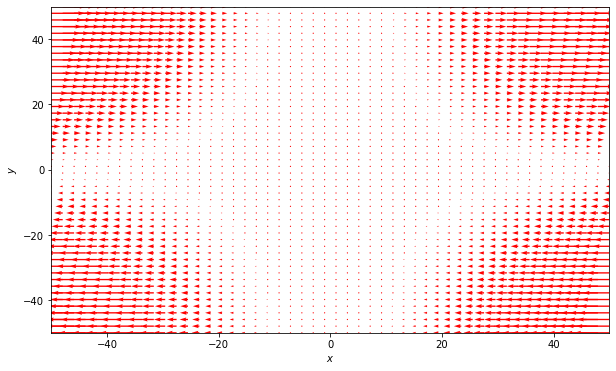
\includegraphics[scale=.5]{diagrama_fase1.png}
	\end{figure}

	\begin{tcolorbox}[colback=gray!5!white,colframe=gray!75!black]
		\textbf{\large{(h)}} On considère maitenant $f(x,y) = (x^2 - yx^4, 0)$. Soit $a>0$, montrer que l'on a $T_{max}(a,0) < +\infty$ alors que pour tout $\epsilon$ tel que $\epsilon a^2 < 1$, on a $T_{max}(a, \epsilon) = +\infty$.
		
		Ceci peut s'écrire
		\[\lim_{\epsilon \to 0} T_{max}(a, \epsilon) \not= T_{max}(a,0)\]
	\end{tcolorbox}

	Si $y_0 = 0$, on note que 
	
	\begin{align}
		\dot{x}(t) &= x^2\\
		\iff \frac{dx}{x^2} &= dt \quad \text{similaire à l'équation de l'exercice 1g} \\
		\iff x(t) &= \frac{x_0}{1 - x_0t}
	\end{align}
	
	Donc, $T_{max}(a, 0) = \frac{1}{a} < +\infty$.
	
	Alors, soit $y_0$ tel que $y_0x_0^2 < 1$.
	
	On note que
	
	\begin{align}
		\dot{x}(t) &= x^2 - y_0x^4\\
		\iff \frac{dx}{x^2(1 - y_0x^2)} &= dt\\
		\iff dx \left(\frac{1}{x^2} + \frac{y_0}{1 - y_0x^2} \right) &= dt\\
		\iff \int_{x_0}^{x(t)} dx \left(\frac{1}{x^2} + \frac{y_0}{1 - y_0x^2} \right) &= \int_{0}^{t} dt
	\end{align}
	
	Avec la substitution $u = x_0\sqrt{y_0}$
	
	\begin{align}
		\int_{x_0}^{x(t)} \frac{y_0}{1 - y_0x^2} dx &= \int_{x_0\sqrt{y_0}}^{x(t)\sqrt{y_0}} \frac{y_0}{1 - u^2} \frac{du}{\sqrt{y_0}}\\
		&= \frac{\sqrt{y_0}}{2}\left(\int_{x_0\sqrt{y_0}}^{x(t)\sqrt{y_0}} \frac{1}{1+u} + \frac{1}{1-u}\right)\\
		&= \frac{\sqrt{y_0}}{2}(\log(1 + x(t)\sqrt{y_0}) + \log(1 - x(t)\sqrt{y_0}) - \log(1 + x_0\sqrt{y_0}) - \log(1 - x_0\sqrt{y_0}))
	\end{align}
	
	On note que $\log(1 - x_0\sqrt{y_0})$ est bien définie car $x_0\sqrt{y_0} < 1$.
	
	Donc,
	
		\[-\frac{1}{x(t)} + \frac{1}{x_0} + \frac{\sqrt{y_0}}{2}\log\left(\frac{1 - x(t)^2y_0}{1-x_0^2y_0}\right) = t\]
	
	On note que $|x(t)| < \frac{1}{y_0}$. Donc, la solution est globale.
	
	\[T_{max}(a, \epsilon) = + \infty\]


	\subsection*{Exercice 2}
	
	\begin{tcolorbox}[colback=red!5!white,colframe=red!75!black]
		Pour $A \in M_n(\mathbb{R})$, la suite $\sum_{k=0}^{N} \frac{A^k}{k!}$ (avec $A^0 = I_n$ la matrice identité) est une suite de Cauchy et converge vers une matrice notée $e^A$. Si de plus $A$ et $B$ dans $M_n(\mathbb{R})$ commutent, alors on a $e^Ae^B = e^{A+B} = e^Be^A$.
	\end{tcolorbox}

	\begin{tcolorbox}[colback=gray!5!white,colframe=gray!75!black]
		\textbf{\large{(a)}} Soit $A \in M_n(\mathbb{R})$ et $f:\mathbb{R} \to M_n(\mathbb{R})$ définie par $f(t) = e^{tA}$. Montrer que $f$ est de classe $\mathcal{C}^1$ et calculer sa dérivée. 
	\end{tcolorbox}
	
	On veut montrer que $||e^{A}|| \leq e^{ ||A||}$.
	
	\begin{align}
		||e^A|| &= || \sum_{k=0}^{+\infty} \frac{A^k}{k!}||\\
		&\leq \sum_{k=0}^{+\infty} \frac{||A^k||}{k!}\\
		&\leq \sum_{k=0}^{+\infty} \frac{||A||^k}{k}\\
		&= e^{||A||}
	\end{align}
	
	Alors, on veut montrer que $f$ est continue. $\forall t_0 \in \mathbb{R} \quad \forall \epsilon > 0$, on pose 
	
	\[\delta = \frac{\ln(\epsilon)}{||A||}\]
	
	Soit $t \in \mathbb{R}$ tel que $| t - t_0 | < \delta$, on a
	
	\begin{align}
		|| f(t) - f(t_0)|| &= || e^{(t-t_0)A}||\\
		&\leq ||e^{\delta A}||\\
		&\leq e^{|| \delta A||}\\
		&= e^{||A|| \cdot \frac{\ln(\epsilon)}{||A||}}\\
		&= \epsilon
	\end{align}
	
	On veut calculer $\forall t \in \mathbb{R}$ la limite 
	
	\begin{align}
		\lim_{h \to 0} \frac{f(t+h) - f(t)}{h} &= \lim_{h \to 0} \frac{e^{A(t+h)} - e^{At}}{h} \\
		&= \lim_{h \to 0} \frac{e^{Ah}}{h}\\
		&= \lim_{h \to 0} \frac{1}{h} \sum_{k = 0}^{+\infty} \frac{1}{k!} (Ah)^k\\
		&= \lim_{h \to 0} A \sum_{k = 0}^{+\infty} \frac{1}{k!} (Ah)^k \\
		&= A e^{At}
	\end{align}
	
	Donc $f'(t)$ existe et on note que $f'(t) = Ae^{tA}$ est continue car $f(t)$ est continue.
	

	\begin{tcolorbox}[colback=gray!5!white,colframe=gray!75!black]
		\textbf{\large{(b)}}Soit $f:\mathbb{R} \to M_n(\mathbb{R})$ une application de classe $\mathcal{C}^1$ telle que $f(s+t) = f(s)f(t)$ pour tous $s,t \in \mathbb{R}$ et telle que $f(0)$ est inversible. Montrer qu'il existe une matrice $A \in M_n(\mathbb{R})$ telle que $f(t) = e^{tA}$ pout tout $t \in \mathbb{R}$.
	\end{tcolorbox}

	On note que $f'(t) = f'(0)f(t)$.
	
	Soit $f'(0) = A \in M_n(\mathbb{R}) \quad \implies \quad  f(t) = e^{tA} \quad \forall t \in \mathbb{R}$ est solution globale.
	
\end{document}